\renewcommand\MaCouleur{Orange}
\chapter{Tableaux}
\thispagestyle{empty}

\section{Composer un tableau}
\subsection{Créer des lignes et des colonnes}

Pour créer un tableau, aucun package supplémentaire n'est chargé.
L'environnement \NomEnv{tabular} sera utilisé en spécifiant un argument obligatoire composé d'une des trois lettres suivantes : \ordi l, \ordi c ou \ordi r. On peut inscrire plusieurs de ces lettres et une même lettre peut apparaître plusieurs fois.

Le nombre de lettres inscrites correspond simplement au nombre de colonne que contiendra le tableau. Dans chacune des colonnes, le texte pourra alors être aligné à gauche (\ordi l), centré (\ordi c) ou aligné à droite (\ordi r). Les lettres sont des \jargon{spécificateurs de colonnes}.

Ainsi, l'instruction \NomCom{begin}\ordi{\{tabular\}\{rcl\}} permettra la création d'un tableau contenant trois colonnes, dont le texte sera aligné à droite dans la première colonne, centré dans la deuxième et enfin aligné à gauche dans la troisième. Il est inutile de spécifier le nombre de lignes.\bigskip

{\NewFont
\begin{SideBySideExample}
    \begin{tabular}{rcl}
        Article & Couleur & Prix en euros \\[0.5cm]
        Pantalon & bleu & 25 \\
        Gants & blanc & 15 \\
            & Total & 40
    \end{tabular}
\end{SideBySideExample}
}\bigskip

Comme pour l'environnement \NomEnv{align}, \verb!&! spécifie l'emplacement de l'alignement : autrement dit ce symbole sépare chaque colonne, y compris les colonnes vides.

La commande de changement de ligne \verb!\\! admet un argument optionnel qui sert à indiquer l'espace verticale que l'on veut insérer après cette ligne.

Afin de mieux visualiser les différentes lignes et colonnes, on peut ajouter des \jargon{filets} : la commande \NomCom{hline} trace un \jargon{filet horizontal}.
Pour insérer un \jargon{filet vertical}, on peut inscrire une barre verticale \verb!|! entre les deux spécificateurs de colonnes concernés.\bigskip

{\NewFont
\begin{SideBySideExample}
    \begin{tabular}{r||c|l}
        Article & Couleur & Prix en euros \\ \hline\hline
        Pantalon & bleu & 25 \\
        Gants & blanc & 15 \\ \hline
          & Total & 40
    \end{tabular}
\end{SideBySideExample}
}

\subsection{Fusionner des colonnes}

\LaTeX{} offre la commande \NomCom{multicolumn}\ArgObl{nombre-colonnes}\ArgObl{specificateur}\ArgObl{texte} qui permet de fusionner horizontalement des colonnes.\bigskip

{\NewFont
\begin{SideBySideExample}
    \begin{tabular}{r|c|l}
        \multicolumn{1}{c|}{Article} &
        Couleur & Prix en euros \\ \hline
        Pantalon & bleu & 25 \\
        Gants & blanc & 15 \\ \hline
        \multicolumn{2}{r}{Total :} & 40
    \end{tabular}
\end{SideBySideExample}
}\bigskip

\begin{info}
    On constate dans l'exemple précédent que la commande \NomCom{multicolumn} permet non seulement de fusionner plusieurs colonnes mais aussi de modifier ponctuellement le spécificateur de colonne sur une cellule en particulier.
\end{info}

\subsection{Spécificateurs de colonne supplémentaires}

Les trois spécificateurs de base ne permettent pas de changement de ligne au sein d'une même cellule. De plus, on ne peut pas spécifier la largeur de la cellule. Le spécificateur \ordi{p}\ArgObl{dim} permet de composer une colonne en imposant une largeur : le texte est alors composé comme un paragraphe normal. \bigskip

{\NewFont
\begin{SideBySideExample}
    \begin{tabular}{r|p{4.5cm}}
        Rectangle & Quadrilat\`ere dont les diagonales
        sont de m\^eme longueur et
        se coupent en leur milieu.\par
        Le rectangle est un parall\'elogramme.
    \end{tabular}
\end{SideBySideExample}
}\bigskip

Dans l'exemple précédent, on constate que les deux paragraphes sont alignés sur le haut de la cellule. On pourrait avoir envie de centrer verticalement ces paragraphes. On utilisera simplement \ordi{m}\ArgObl{dim} :\bigskip

{\NewFont
\begin{SideBySideExample}
    \begin{tabular}{r|m{4.5cm}}
        Rectangle & Quadrilat\`ere dont les diagonales
        sont de m\^eme longueur et
        se coupent en leur milieu.\par
        Le rectangle est un parall\'elogramme.
    \end{tabular}
\end{SideBySideExample}
}\bigskip

\begin{info}
    Dans l'exemple précédent, remplacer \ordi{m\{4.5cm\}} par \ordi{b\{4.5cm\}}. Que se passe-t-il ?
\end{info}

\subsection*{\ExoFiche}
Comment composer le tableau suivant  sachant que les deux colonnes extérieures mesurent $\np[cm]{2}$ alors que la colonne centrale mesure $\np[cm]{8}$ ?\bigskip

\begin{CadreExemple}
    \begin{center}
        \begin{tabular}{|m{2cm}|m{8cm}|m{2cm}|}
        	\hline
        		\centering 1\iere \textsc{s} & \centering  Jeudi 13 novembre \np{2014} & \centering \textbf{\'Etude de fonctions} \tabularnewline
        	\hline
        		\multicolumn{3}{|c|}{\textsc{Contrôle de mathématiques}} \\
        	\hline
                \multicolumn{1}{|r}{\textsc{Nom}:} & \multicolumn{2}{l|}{} \\
        		\multicolumn{1}{|r}{Prénom:} & \multicolumn{2}{l|}{} \\
        	\hline
                \multicolumn{3}{|l|}{\bfseries Note et observations :} \\[1cm]
            \hline
        \end{tabular}
    \end{center}
\end{CadreExemple}

\begin{info}
    On pourra regarder avec beaucoup d'attention la documentation du package \NomPack*{tabularx} qui offre l'environnement \NomEnv*{tabularx} qui permet de spécifier la largeur total du tableau et donc de calculer ensuite automatiquement la largeur de colonnes spécifiques.
\end{info}

\section{Les tableaux en mathématiques}
\subsection{L'environnement {\normalsize\textit{\textsf{array}}}}

Comme nous allons rapidement le voir, il peut être utile de composer des tableaux en mode mathématique (notamment en mode hors texte). Dans ce cas, on utilise dans ce mode l'environnement \NomEnv{array} qui fonctionne comme \NomEnv{tabular} pour les commandes expliquées dans la section précédente.\bigskip

{\NewFont
\begin{SideBySideExample}
    \[\begin{array}{rcl}
        f \colon \R & \rightarrow & \R_+ \\
                    x & \mapsto & x^2
    \end{array}\]
\end{SideBySideExample}
}\bigskip

\subsection{Les systèmes}

On avait constaté l'utilité des symboles étirables verticalement à l'aide de \NomCom{left} et \NomCom{right}. Servons-nous de \NomCom{left}\verb!\{! pour créer une grande accolade pour les systèmes :\bigskip

{\NewFont
\begin{SideBySideExample}
    \[\left\{
    	\begin{array}{ccccccl}
    		2x & - & y & - & 3z & = & 1 \\
    		3x & + & 2y &  &  & = & -4 \\
    		-x &  &  & + & 6z & = & 22
    	\end{array}
    \right.\]
\end{SideBySideExample}
}\bigskip

\begin{info}
    \NomCom{left} et \NomCom{right} fonctionnent toujours ensemble. Ici, on ne veut qu'une accolade à gauche. On utilise donc \NomCom{left}\ordi{\symbol{92}\{} mais la commande \NomCom{right.} est nécessaire pour que la compilation ait lieu sans erreur.
\end{info}

{\NewFont
\begin{SideBySideExample}
    \[\lvert x \rvert =
    \left\{
    	\begin{array}{cl}
    		-x & \text{si } x < 0 \\
    		x & \text{sinon}
    	\end{array}
    \right.\]
\end{SideBySideExample}
}\bigskip

\subsection{Les matrices}

Cette fois-ci, on peut penser à utiliser \NomCom{left(} et \NomCom{right)}\dots\bigskip

{\NewFont
\begin{SideBySideExample}
    \[M = \left(
    	\begin{array}{ccc}
    		2 & -1 & 0 \\
            3 & 4 & 1 \\
            0 & 2 & 3
    	\end{array}
    \right)\]
\end{SideBySideExample}
}\bigskip

\dots mais en réalité des environnements spécifiques existent pour l'écriture des matrices. Entre autre, on retiendra les environnements \NomEnv{pmatrix} et \NomEnv{vmatrix} ainsi que la commande \NomCom{bordermatrix}.\bigskip

{\NewFont
\begin{SideBySideExample}
    \[M =
    	\begin{pmatrix}
    		2 & -1 & 0 \\
            3 & 4 & 1 \\
            0 & 2 & 3
    	\end{pmatrix}
    \]\medskip
    \[\det(M) =
    	\begin{vmatrix}
    		2 & -1 & 0 \\
            3 & 4 & 1 \\
            0 & 2 & 3
    	\end{vmatrix} = 29
    \]\medskip
    \[
        \bordermatrix{
            & f(e_1) & f(e_2) \cr
        e_1 & 1 & 2 \cr
        e_2 & 0 & 3 \cr}
    \]
\end{SideBySideExample}
}\bigskip

\section{Tableaux de signes et tableaux de variations}

Ici nous allons utiliser l'environnement \NomEnv{tikzpicture} du package \NomPack{TikZ}. Nous ne dirons rien sur ce package pour le moment mais nous reviendrons dessus lorsque nous traiterons les graphiques. Cependant, pour créer des tableaux de signes et des tableaux de valeurs, Alain \textsc{Matthes} a créé le package \NomPack{tkz-tab} qui répond parfaitement bien à notre problème. Il faut donc penser dès à présent à ajouter \verb!\usepackage{tkz-tab}! au préambule.

\begin{info}
    Selon l'installation effectuée, il est possible que \NomPack*{tkz-tab} ne soit pas présent dans votre distribution. Vous vous en rendrez rapidement compte en compilant le premier exemple. La documentation de ce package est également une source à consulter absolument.
\end{info}

\subsection{Tableaux de signes}

{\NewFont
\begin{CenterExample}
    \textbf{Tableau de signes :}\par
    \begin{tikzpicture}
        \tkzTabInit[nocadre,espcl=1.5]%
            {$x$/0.75,Signe de \\ $x+2$/1.5,Signes de \\ $x^2-1$/1.5,%
            signe du \\ produit/1.5,signe du \\ quotient/1.5}%
            {$-\infty$,$-2$,$-1$,$1$,$+\infty$}
        \tkzTabLine{,-,z,+,t,+,t,+}
        \tkzTabLine{,+,t,+,z,-,z,+}
        \tkzTabLine{,-,z,+,z,-,z,+}
        \tkzTabLine{,-,z,+,d,-,d,+}
    \end{tikzpicture}
\end{CenterExample}
}\bigskip

Un tableau de signes ou de variations commencera toujours par \NomCom{tkzTabInit} dont voilà la syntaxe :
\begin{center}
    \NomCom{tkzTabInit}\ArgOpt{options}\ArgObl{première colonne}\ArgObl{première ligne}
\end{center}

 En option est spécifié que le cadre autour du tableau ne doit pas être dessiné et que l'espace entre les valeurs de la première ligne est réglée par le paramètre \verb!espcl!.

 Ensuite, on énumère les différentes lignes de la première colonne : \Arg{nom de la ligne}\verb!/!\Arg{hauteur de la ligne}. Le \Arg{nom de la ligne} accepte des changements de lignes à l'aide de \verb!\\! et on passe d'une ligne à l'autre en utilisant la virgule.

 Enfin, dans le dernier argument, on écrit les valeurs de la première ligne en les séparant par une virgule.\medskip

 Pour finir, pour chaque ligne, on écrit les signes par la commande \NomCom{tkzTabLine}. La lettre \verb!t! crée un filet vertical en pointillés et la lettre \verb!z! fait la même chose en ajoutant un zéro. La lettre \verb!d! insère une double-barre pour les valeurs interdites.

 \begin{info}
    Si on a besoin d'écrire des nombres décimaux, on prendra soin de les écrire entre accolades pour que la virgule ne crée pas de conflit : \ordi{\$\{1,5\}\$}.
 \end{info}

 \subsection{Tableaux de variations}

 {\NewFont
\begin{CenterExample}
    \textbf{Tableau de variations :}\par
     \begin{tikzpicture}
        \tkzTabInit[nocadre,espcl=2]{$x$/0.75,Variations \\ de $f(x)$/1.75}{$-3$,$-1$,$1$,$4$}
        \tkzTabVar{+/$6$,-D+/$-\infty$/$+\infty$,-/,+/$-5$}
    \end{tikzpicture}
\end{CenterExample}
}\bigskip

Il nous suffit ici de commenter la commande \NomCom{tkzTabVar} : pour chaque valeur de $x$ indiquée sur la première ligne, on peut préciser une valeur précédée du symbole \verb!+/! pour dire que la valeur sera écrite <<~en haut~>> ou bien \verb!-/! pour dire que la valeur sera écrite << en bas >>. Des flèches relieront alors automatiquement les différentes valeurs :
\begin{center}
    \NomCom{tkzTabVar}{\tt\{}\Arg{+ ou -}{\tt/}\Arg[1]{valeur} , \Arg{+ ou -}{\tt/}\Arg[2]{valeur} , ...{\tt\}}
\end{center}

\begin{info}
    Pour la double-barre avec des valeurs indiquées avant et après celle-ci, on notera :\par {\tt -D+/\Arg*[1]{valeur}/\Arg*[2]{valeur}} ou bien {\tt +D-/\Arg*[1]{valeur}/\Arg*[2]{valeur}}.
\end{info}

\subsection{Un mélange}
Et voilà maintenant ce que l'on peut obtenir :

 {\NewFont
\begin{CenterExample}
    \begin{tikzpicture}
        \tkzTabInit[nocadre,espcl=2]%
            {$x$/0.75,signe de \\ $f'(x)$/1.5,Variations \\ de $f(x)$/1.75}%
            {$-3$,$-1$,$1$,$4$}
        \tkzTabLine{,+,z,-,z,+}
        \tkzTabVar{-/$-\infty$,+/,-/,+/$+\infty$}
    \end{tikzpicture}
\end{CenterExample}
}


\section{Exercices}
\subsection*{\ExoFiche}
Comment obtenir le \textsc{q.c.m.} suivant ?\medskip

\begin{CadreExemple}
\begin{center}
\begin{tabular}{|c|c|c|c|}
\hline
 & Réponse A & Réponse B & Réponse C \\
\hline\hline
 \textbf{Question 1.} & 1a & 1b & 1c \\
\hline
 \textbf{Question 2.} & 2a & 2b & 2c \\
\end{tabular}
\end{center}
\end{CadreExemple}

\subsection*{\ExoFiche}

Composer le code source de l'énoncé suivant puis taper la correction.\medskip

\begin{CadreExemple}
\textbf{Exercice.}\par
    On considère la fonction $f$ définie de la façon suivante :
        \[\begin{array}{rcl}
        f \colon \R & \rightarrow & \R \\[5pt]
                    x & \mapsto & \frac 13 x^3 + x^2 - 3x + 4
    \end{array}\]
    \begin{enumerate}
        \item Déterminer la dérivée $f'$ de $f$ sur $\R$.
        \item Déterminer les racines de $f'$.
        \item À l'aide du tableau de signes de $f'$, dresser le tableau de variations de $f$ sur $\R$.
    \end{enumerate}
\end{CadreExemple}


\section{Complément : le tableur}

Le package \NomPack{pas-tableur} de Stéphane \bsc{Pasquet} permet d'imiter l'apparence d'un tableur. Cependant, il n'effectue pas de calcul automatique comme dans un tableur (pour cela, on pourra jeter un {\oe}il sur le package \NomPack{spreadtab}). Une fois encore, ce package utilise \NomPack{TikZ} et son environnement \NomEnv{tikzpicture}.

La première commande à retenir est la suivante :
\begin{center}
    \NomCom{tableur}\ArgOpt{nombres-lignes}\ArgObl{colonnes}
\end{center}

L'argument \Arg{colonnes} permet de spécifier les lettres des colonnes utilisées soit une par une, soit en utilisant un << intervalle >>.
Ensuite, \begin{center}\NomCom{celtext}\ArgOpt{options}\ArgObl{colonne}\ArgObl{ligne}\ArgObl{texte}\end{center} permet d'écrire un texte dans la cellule définie par \Arg{colonne} et \Arg{ligne}. Parmi les options, \verb!l!, \verb!c! et \verb!r! sont utilisées pour l'alignement du texte. Des formules commençant par le signe \verb!=! peuvent être écrites et le texte peut être mis en forme en utilisant les commandes correspondantes.

Et enfin, les commandes \NomCom{selecCell} et \NomCom{multiSelec} permettent de mettre en couleur des cellules sélectionnées. Les exemples suivants vous montrent comment :\bigskip

{\NewFont
\begin{SideBySideExample}
    \begin{tikzpicture}
        \tabcolwidth{1cm}
        \tableur{A,D,T}
    \end{tikzpicture}\bigskip

    \begin{tikzpicture}
        \tabcolwidth{2cm}
        \tableur[3]{A,B,C}
        \multiSelec{A-2}{B-3}
    \end{tikzpicture}\bigskip

    \begin{tikzpicture}
        \tabcolwidth{1.5cm}
        \tableur[3]{A-D}
        \celtxt[c]{A}{1}{\itshape x}
        \celtxt[r]{A}{2}{0}
        \celtxt[r]{A}{3}{1}
        \celtxt[c]{B}{1}{\itshape f(x)}
        \celtxt{B}{2}{=A2*A2}
        \selecCell{B}{2}
    \end{tikzpicture}
\end{SideBySideExample}
}
